
\section{Marketing und Vertrieb}
\subsection{Ausgangslage und Positionierung}
\ac{KARL} Diagnostics adressiert die steigende Komplexität moderner Fahrzeuge, die Verdichtung von Serviceprozessen und den anhaltenden Fachkräftemangel in Kfz-Werkstätten mit einer \ac{E2E}-Diagnoselösung, die \ac{OBD}-II/\ac{CAN}-Hardware und KI-gestützte Software verbindet (Priorisierung, geführte Prüfpläne, Teile- und Reparaturempfehlungen, perspektivisch DMS-Integration). Die Positionierung fokussiert auf präzise Erstdiagnosen, eine höhere \ac{FTFR} sowie messbare Prozesssicherheit in der Annahme und Werkstattabwicklung. Die Lösung differenziert sich durch \ac{OTA}-Updates, \ac{KI}-gestützte Fehlerpriorisierung und einen klaren Pfad zur Integration in bestehende Systeme der Werkstatt-IT \citep[vgl.][o.S.]{market-analytics-2025}.

\subsection{Business Model Canvas}
\textbf{Customer Segments}\\
\ac{KARL} adressiert primär professionelle Akteure im europäischen Kfz‑Aftermarket mit hoher Prozess- und Ergebnisverantwortung. Dazu gehören freie Werkstätten, markengebundene Servicebetriebe, Serviceketten sowie mobile Mechaniker, die markenübergreifende Diagnostik, kurze Durchlaufzeiten und verlässliche Erstbehebungsraten benötigen. Perspektivisch ist eine internationalisierte Ausweitung nach Westeuropa, Nordamerika und China vorgesehen, sobald Referenzen, Lokalisierungen und Integrationen in den Zielregionen belastbar vorliegen. Die verschiedenen Kundengruppen haben unterschiedliche Anforderungen: Kleine Werkstätten achten vor allem auf Kosten und einfache Bedienung. Werkstattketten legen Wert auf Skalierbarkeit und einheitliche Abläufe.\\

\textbf{Value Propositions}\\
Der Kernnutzen liegt in präziser, erklärbarer Erstdiagnose mit durchgängiger Prozessführung: \ac{OBD}‑II/\ac{CAN}‑fähige Hardware verbindet das Fahrzeug robust mit \ac{CARL} und \ac{KARLA}, wo \ac{KI}‑gestützte Fehlerpriorisierung, geführte Prüfpläne und Teileempfehlungen bereitgestellt werden. Das ganze System wird noch durch \ac{OTA}‑Updates ergänzt. Für Werkstätten wird damit Zeitdruck in der Annahme reduziert, die \ac{FTFR} erhöht und der Teiletausch „auf Verdacht“ durch strukturierte Ursachenanalyse ersetzt. Die Diagnosen werden nachvollziehbar, da Hypothesen, Wahrscheinlichkeiten und Begründungen transparent ausgegeben werden und jeder bestätigte Fall die Wissensbasis verbessert. Im Wettbewerb differenziert sich \ac{KARL} gegenüber teuren, komplexen Premium‑Testern und \ac{OEM}‑gebundenen Tools über Herstellerunabhängigkeit, geführte Prüfpfade, explainable AI sowie die Verbindung aus lernender Wissensbasis und pragmatischer Plug‑and‑Play‑Integration in bestehende Werkstattprozesse.\\

\textbf{Channels}\\
Der Marktzugang kombiniert direkten \ac{B2B}‑Vertrieb (Demos und Teststellungen) mit Partnerkanälen über Werkstattausrüster, Distributoren und Systemintegratoren, um Reichweite, Logistik und regionale Präsenz aufzubauen. Digitale Kanäle stützen den Funnel mit Content Marketing (Leitfäden, Fallstudien, \ac{DTC}‑Bibliotheken), Webinaren und Fachportalen. Messen und Verbandsarbeit erhöhen die Glaubwürdigkeit in konservativen Beschaffungsprozessen, während Zertifizierungen die Anwenderkompetenz sichern. Die Software wird cloudbasiert ausgeliefert und gepflegt und erhält \ac{OTA} Updates. Die Hardware wird über eine Partnerlogistik bereitgestellt. Der Rollout startet in der DACH-Region und wird anschließend auf Westeuropa ausgeweitet. \\

\textbf{Customer Relationships} \\
Wir begleiten unsere Kunden Schritt für Schritt. Von der Einführung bis zur langfristigen Nutzung erhalten unsere Kunden immer Unterstützung. Neue Kunden erhalten strukturierte Onboardings mit Schulungen um eine fehlerfreie Verwendung von KARL zu ermöglichen.Unser Customer-Success-Team sorgt dafür, dass die Software intensiv genutzt wird, Kunden als Referenzpartner gewonnen werden und Rückmeldungen direkt in die Weiterentwicklung einfließen. Dabei helfen klare Kennzahlen wie Akquisekosten, Conversion-Raten, Umsatzbindung und Kündigungsquote, um alle Phasen – von der ersten Nutzung bis zur Erweiterung – datenbasiert zu steuern. Zertifizierungen und Community-Formate sollen in der Zukunft umgesetzt werden um den Austausch von Best Practices zu fördern, denn so kann Vertrauen in KI-gestützte Empfehlungen gewonnen werden. \\

\textbf{Revenue Streams} \\
\ac{KARL} nutzt ein hybrides Modell: einmalige Hardwareerlöse aus \ac{OBD}/\ac{CAN}‑Interfaces und Zusatzsensorik sowie wiederkehrende \ac{SaaS}‑Lizenzen pro Arbeitsplatz mit gestaffelten Funktionsumfängen (z.B. Priorisierung, erweiterte Daten/Empfehlungen, Integrationen, \ac{SLA}). Ergänzende Ertragsquellen sind Schulungen/Zertifizierungen, Integrationsprojekte und Premium‑Support. Die Preispolitik ist nutzenbasiert und reflektiert Effizienzgewinne (Zeit, Erstbehebung, Teiletrefferquote) sowie die Skaleneffekte der Wissensbasis. Damit verlagert sich der Umsatzmix mit wachsender Traktion hin zu margenstarken Lizenzerlösen, während die Hardware als Enabler dient und den Geräte‑Lock‑in für stabile Nutzung sicherstellt. \\

\textbf{Key Resources} \\
Wesentliche Ressourcen sind der Diagnose‑Stack (\ac{OBD}/\ac{CAN}‑Anbindung, Datenmodelle), die Cloud‑/Mobile‑Plattform (\ac{CARL}/\ac{KARLA}), proprietäre \ac{KI}‑Modelle mit erklärbarer Ausgabenlogik und eine wachsende Wissensbasis aus realen, anonymisierten Fällen. Hinzu kommen Integrationsassets (APIs, Konnektoren), Telemetrie/Monitoring, Marken‑ und Vertriebskanäle sowie das qualifizierte, funktionsübergreifende Team (Fullstack‑Entwickler, Data Engineers/Scientist, Vertrieb, Einkauf/QS), das die Brücke zwischen Feldanforderungen und Produktinkrementen schließt. Partnerschaften mit Fertigern, Distributoren, \ac{DMS}/Telematik‑Anbietern und Cloud/Datenpartnern sind teil‑externe Ressourcen, die Lieferfähigkeit, Integrationstempo und Skalierung operativ absichern. \\

\textbf{Key Activities}\\
Im Zentrum stehen Entwicklung und Betrieb der Plattform mit kurzen Release‑Zyklen, \ac{CI/CD}, \ac{OTA}‑Update‑Mechanismen und Telemetrie gestützter Qualitätssicherung, ergänzt um Datenaufnahme, Harmonisierung, Validierung und Modelltraining samt Monitoring im Feld. Go to Market   Aktivitäten umfassen Vertrieb (Demos, Teststellungen), Partnerenablement (Co‑Marketing, Schulungen), Onboarding/Customer Success sowie Zertifizierungen zur Kompetenzsicherung. Einkauf und Qualitätssicherung managen die externe Hardwarefertigung, Zweitquellen, Prüf- und Abnahmeprozesse sowie Änderungswesen, um Serienqualität, Verfügbarkeit und Kostenstabilität sicherzustellen. \\

\textbf{Key Partnerships}\\
Für Reichweite und Liefersicherheit stützt sich \ac{KARL} auf Werkstattausrüster/Distributoren, die Zugang zum \ac{IAM}‑Netz und etablierte Logistikketten bieten, sowie auf Fertigungspartner für \ac{OBD}/\ac{CAN}‑Hardware mit geprüften Qualitätsprozessen und Zweitquellenstrategie. Integrationspartner im Bereich \ac{DMS}/Telematik und Cloud/Datenanbieter beschleunigen die Inbetriebnahme und senken Projekt‑ und Betriebsrisiken. Ausbildungs‑ und Schulungspartner sichern eine flächige Qualifizierung der Anwender. Verbandsarbeit und Messen dienen als Glaubwürdigkeits‑ und Akquisitionshebel in einem konservativen Beschaffungsumfeld und erleichtern Referenzaufbau in Zielsegmenten. \\

\textbf{Cost Structure} \\
Die Kostenstruktur umfasst F\&E für Embedded/Software/\ac{KI}, Cloud‑ und Datenbetrieb, externe Hardwarefertigung/Logistik, Go‑to‑Market (Marketing, Vertrieb, Partner), Customer Success/Support sowie Qualitätssicherung und Zuliefereraudits. Skaleneffekte in Einkauf/Fertigung und Automatisierung im Onboarding/Support (Self‑Service, In‑App‑Hilfen) senken Stück- und Servicekosten. Mit steigender Nutzerbasis verbessert sich der Deckungsbeitrag der \ac{SaaS}‑Komponente, während Hardware gezielt margenschonend als Wachstumstreiber eingesetzt wird. Regelmäßige Portfolio‑ und \ac{SLA}‑Reviews sichern die Balance aus Funktionsausbau, Betriebsstabilität und Kostenkontrolle entlang der Rollout‑Phasen (DACH → Westeuropa). \\

\subsection{Das Magische Dreieck des Geschäftsmodells}

\textbf{Ausgangspunkt und Zweck}\\
Das Magische Dreieck beschreibt ein Geschäftsmodell entlang von vier miteinander verknüpften Dimensionen: Zielkunde (Wer?), Nutzenversprechen (Was?), Wertschöpfungskette (Wie?) und Ertragsmechanik (Wert?). Änderungen an einer Ecke bedingen stets Anpassungen an den anderen, weshalb die vier Bausteine als integriertes System zu gestalten sind. Für KARL Diagnostics dient das Dreieck dazu, die herstellerunabhängige Diagnoselösung präzise auf Werkstattpraxis, skalierbare Bereitstellung und belastbare Finanzierung auszurichten, ohne den Kundennutzen aus dem Blick zu verlieren.\\

\textbf{Wer? Zielkunden}\\
Im Zentrum stehen freie und markengebundene Werkstätten, Serviceketten sowie mobile Mechaniker in DACH und Westeuropa. Die Segmentlogik unterscheidet nach Kaufkriterien: \ac{SMB}‑Werkstätten priorisieren Bedienbarkeit und TCO, Ketten benötigen standardisierte, skalierbare Abläufe. DDer Rollout startet in der DACH-Region und wird anschließend auf Westeuropa ausgeweitet. \\

\textbf{Was? Nutzenversprechen}\\
KARL liefert präzise, erklärbare Erstdiagnosen durch die Kombination OBD/CAN‑Hardware mit \ac{CARL} und mobiler App \ac{KARLA}: \ac{KI}‑gestützte Fehlerpriorisierung, geführte Prüfpläne, Teileempfehlungen, \ac{OTA}‑Updates und Offline‑Fähigkeit, eingebettet in bestehende Werkstattprozesse. Der messbare Kundennutzen umfasst höhere \ac{FTFR}, kürzere Standzeiten, weniger Teiletausch auf Verdacht sowie auditierbare Prozessqualität. Die erklärbare Ausgabe und das kontinuierliche Lernen aus anonymisierten Fällen stärken Vertrauen und Effektivität und ist ein entscheidendes Hilfsmittel in der Zeit des Fachkräftemangels. \\

\textbf{Wie? Wertschöpfungskette}\\
Die Wertschöpfung kombiniert Hardwarebeschaffung und QS, Datenaufnahme über OBD/CAN und Zusatzmessgeräte, Cloud‑Verarbeitung mit Datenharmonisierung, Modelltraining und Telemetrie‑basiertem Monitoring sowie die Auslieferung von Funktionen via \ac{CI/CD} und \ac{OTA}. Go‑to‑Market und Service werden über direkten \ac{B2B}‑Vertrieb, Partnernetze (Werkstattausrüster, Distributoren, Systemintegratoren), strukturiertes Onboarding, Schulungen und Customer Success skaliert. Integrationspartner (\ac{DMS}/Telematik) beschleunigen die Inbetriebnahme und senken Projektrisiken. \\

\textbf{Wert? Ertragsmechanik}\\
Das Erlösmodell ist hybrid: einmalige Hardwareerlöse für \ac{OBD}/\ac{CAN}‑Interfaces und wiederkehrende \ac{SaaS}‑Lizenzen pro Arbeitsplatz mit Funktions‑ und \ac{SLA}‑Staffelung. Zusätzliche Umsätze entstehen durch Schulungen, Zertifizierungen, Integrationsleistungen und Premium‑Support. Kostenblöcke liegen in F\&E (Embedded/Software/\ac{KI}), Cloud/Datenbetrieb, externer Fertigung/Logistik, Go‑to‑Market und Customer Success. Skaleneffekte in Einkauf/Fertigung sowie Self‑\\Service‑Onboarding und Telemetrie‑gestützter Support verbessern Deckungsbeiträge und verlagern den Umsatzmix hin zu margenstarken Lizenzen. \\

\textbf{Implikationen für die Gestaltung} \\
Da Optimierungen an einer Ecke stets Rückwirkungen erzeugen, muss die Roadmap auf Mehrfachanpassungen ausgelegt werden: Beispielsweise erfordert ein erweitertes Nutzenversprechen (z.B. neue \ac{KI}‑Module) sowohl zusätzliche Daten- und MLOps‑Kapazitäten in der Wertschöpfung als auch eine angepasste Preis-/\ac{SLA}‑Logik in der Ertragsmechanik. Umgekehrt bedingen neue Zielsegmente (z.B. der europäische Markt) andere Integrationen und Nachweise in der Wertschöpfung und rechtfertigen differenzierte Vertrags- und Paketstrukturen im Erlösmodell.\\

\subsection{Marketing-Mix (4P) für KARL}
\textbf{Product}\\
\ac{KARL} umfasst \ac{OBD}-II/\ac{CAN}-Hardware, eine Cloud-Applikation (\ac{CARL}) und eine Mobile App (\ac{KARLA}) für \ac{KI}-gestützte Fehlerpriorisierung, geführte Prüfpläne, Teileempfehlungen und \ac{OTA}-Updates. \\
\textbf{Price}\\
Ein hybrides Hardware-SaaS-Preismodell mit nutzenbasierter Staffelung nach Funktionsumfang, Nutzersitzen und \ac{SLA}\\
\textbf{Place}\\
Go-to-Market über DACH/Westeuropa mit direktem \ac{B2B}-Vertrieb an Werkstätten/Serviceketten/Flotten und Partnern aus dem IAM-Distributionsnetz. Software-Distribution cloudbasiert, Hardware über Partnerlogistik. Zugang zu Fahrzeugdaten und Interoperabilität sind zentrale Faktoren für Reichweite und Skalierung.\\
\textbf{Promotion}\\
Evidenzbasierter Content (Whitepaper, ROI-Cases), Präsenz bei Messen/Verbänden und digitale Lead-Generierung sind wirksam. Kundenzentrierte Demos, Teststellungen und Pilotprojekte sind entscheidend für die Akquise in einem konservativen Beschaffungsumfeld.
\section{Geschäftsmodell und Organisation}
\textbf{Wertlogik und Erlösströme}\\
\ac{KARL} verfolgt ein hybrides Modell aus Hardwareumsatz und wiederkehrenden Softwareerlösen. Die Hardware sorgt für initiale Cashflows, Gerätebindung und robuste Datenaufnahme am Fahrzeug. Die SaaS-Komponente skaliert margenstark über die wachsende Nutzerbasis und regelmäßige Feature-Updates. Ergänzende Services (Schulung, Zertifizierung, Premium-Support, Integration) erhöhen den Kundennutzen und erweitern den Umsatz je Account. Netzwerkeffekte in der Wissensbasis sowie die Datenqualität aus realen Werkstattfällen stärken im Zeitverlauf die Differenzierung und erhöhen die Qualität der Analysen. \\

\textbf{Kostenstruktur und Skalierung}\\
Die Kostenstruktur besteht aus F\&E für \ac{KI}/Software und Embedded, Produktion und Logistik der Hardware, Go-to-Market, Customer Success sowie Cloud-/Datenbetrieb. Skaleneffekte in Fertigung und Einkauf senken Hardware-Stückkosten, während Software mit geringem Grenzkostenanstieg skaliert. Ein klarer Fokus auf Automatisierung (z. B. Self-Service-Onboarding, In-App-Schulungen, Telemetriegestützte Supportpfade) reduziert Servicekosten pro Kunde und erhöht die Bruttomarge im \ac{SaaS}-Anteil auf Dauer. \\

\textbf{Kernprozesse und Qualitätsmanagement}\\
Die Produktentwicklung folgt einem agilen Rahmenwerk mit kurzen Release-Zyklen, kontinuierlichen Updates und enger Einbindung von Pilotkunden. Ein durchgängiges Qualitätsmanagement (Anforderungen, Verifikation, Validierung) stellt Reifegrad, Regeltreue und Servicefähigkeit sicher. Für die Software werden sichere Update-Mechanismen, Telemetrie und Monitoring etabliert. Für die Hardware gilt ein strukturierter Zulieferer- und End-of-Line-Testprozess mit Rückverfolgbarkeit. Dokumentierte Prüfpläne und Wissensartefakte sorgen für konsistente Servicequalität in der Praxis.\\

\textbf{Partnerökosystem und Integration}\\
Technologiepartnerschaften mit Cloud- und Datenanbietern, DMS-Anbindungen, Telematikplattformen sowie Werkstattausrüstern beschleunigen Implementierungen und reduzieren Gesamtrisiken in den Einführungsprojekten. Ein klar definierter Integrationskatalog (APIs, Konnektoren) sowie ein Zertifizierungsprogramm für Implementierungspartner sichern Qualität und Time-to-Value. Strategische Kooperationen mit Ausbildungs- und Schulungspartnern unterstützen die flächendeckende Qualifizierung der Anwender. \\

\textbf{Organisation und Steuerung} \\
Die Organisation ist in der Startphase schlank, cross-funktional und auf schnelle Iteration ausgelegt. Klare Verantwortlichkeiten in Produkt, Engineering, Operations, Vertrieb/Marketing und Customer Success werden durch Objectives and Key Results verbunden. Ein regelmäßiges Entscheidungs- und Risikoreview sichert Priorisierung und Ressourcenallokation entlang von Wachstumszielen. Governance berücksichtigt Datenschutz, IT-Sicherheit und Produktsicherheit, insbesondere im Umgang mit Fahrzeug- und Kundendaten. \\

\textbf{Internationalisierung} \\
Die Expansion verläuft phasenweise: DACH mit Fokus auf Referenzkunden und Prozessstandardisierung, anschließend Westeuropa mit lokaler Anpassung von Content, Datenabdeckung und Integrationen. Lokale Partnernetze, Sprach- und Rechtsraumadaptionen sowie abgestufte Supportmodelle sichern Kundennähe und Servicequalität. Zukünftig ist eine Ausweitung auf Nordamerika und China vorgesehen, sobald die erforderlichen Ressourcen und Partnerschaften etabliert sind. \\
  
\section{Team}
Das Unternehmerteam ist funktionsübergreifend aufgestellt, um die Entwicklung, Skalierung und Markteinführung der Gesamtlösung effizient und mit hoher Umsetzungsqualität voranzutreiben. Die Struktur ist Abbildung \ref{fig:team} zu entnehmen. Wie dort zu erkennen ist sind die Mitarbeiter in drei Teams aufgeteilt welche von den Gründern geleitet werden. Vier Fullstack-Entwickler bestehend aus einem Junior einem Intern und zwei Senior Entwicklern verantworten die Ende-zu-Ende-Softwareentwicklung für die Cloud-Applikation \ac{CARL} und die mobile App \ac{KARLA}, einschließlich Frontend, Backend, API-Design, Sicherheit und Continuous Delivery. Zwei Data Engineers (Junior und Senior) stellen Datenaufnahme, -qualität und -bereitstellung sicher, implementieren robuste Pipelines von der OBD/CAN-Quelle bis in den Cloud-Datenraum und sorgen für verlässliche Betriebsprozesse. Ein Senior Data Scientist entwickelt Diagnose- und Priorisierungsmodelle, evaluiert Modellgüte im Feld und überführt prototypische Verfahren in produktionsreife Services.
\begin{figure}[ht!]
    \centering
    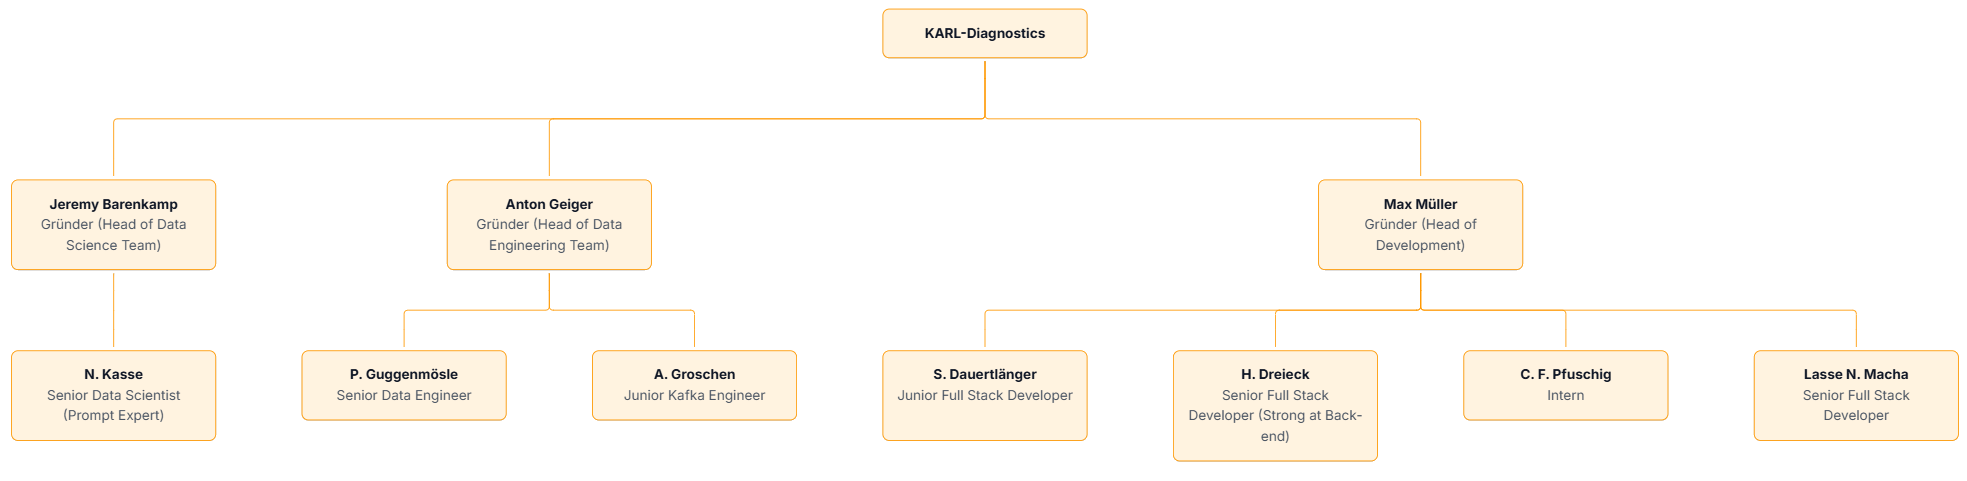
\includegraphics[width=15cm]{images/Our Organization Structure KARL-modified.png}
    \caption{Das KARL-Team}
    \label{fig:team}
\end{figure}

\textbf{Einstellungsfahrplan} \\
Ab dem 10. Monat ist eine größere Erweiterung des Teams geplant. Für den Aufbau des Vertriebs ist eine Einstellung von zwei Vertrieblern geplant. Diese sprechen Pilotkunden und Zielsegmente direkt an, koordinieren Demos, Teststellungen und kommerzielle Angebote und übernehmen die Verantwortung für strukturierte Feedbackschleifen in Richtung Produktentwicklung. Weiter ist ab dem 10. Monat eine Stelle für einen QS-Mitarbeiter geplant. Dieser soll sich primär um den Einkauf und die Qualitätssicherung kümmern. Mit wachsender Traktion werden Teamgrößen in Engineering, Sales und Support skaliert und regionale Vertriebsrollen hinzugefügt. \\

\textbf{Führung und Kultur}\\
Führung fördert Autonomie und Verantwortlichkeit, gestützt durch klare Ziele, belastbare Metriken und hohe Transparenz. Eine Lern- und Feedbackkultur beschleunigt Produktreife und Markterfolg. Kompetenzaufbau wird systematisch über Schulungen, Zertifizierungen und Communities of Practice unterstützt. Incentives kombinieren marktgerechte Vergütung mit Beteiligungsmodellen, die langfristige Wertschöpfung honorieren und die Mitarbeiter motivieren sollen. \\

\textbf{Compliance und Qualifizierung}\\
Für den Einsatz im Automotive-Umfeld werden Qualifizierungen und Standards in Entwicklung, Betrieb und Support verankert. Datenschutz, IT-Sicherheit, sichere Softwarelieferketten sowie rechtliche Rahmenbedingungen beim Datenzugriff und der -verarbeitung sind verbindlicher Bestandteil der Prozesse. Für Anwender werden Schulungs- und Zertifizierungsprogramme etabliert, die Qualität und Sicherheit in der Anwendung fördern sollen.